%==============================================================================
%  LocalRCA -- IEEE conference format (IEEEtran)
%
%  Build:
%     pdflatex localrca_ieee
%     bibtex   localrca_ieee      % only if you switch to a .bib file
%     pdflatex localrca_ieee
%     pdflatex localrca_ieee
%
%  Self-contained: every figure is TikZ/pgfplots, so there are no external
%  image dependencies. Numbers in the figures are the measured values quoted
%  in the text; they are not illustrative.
%==============================================================================
\documentclass[conference]{IEEEtran}
\IEEEoverridecommandlockouts

\usepackage{cite}
\usepackage{amsmath,amssymb,amsfonts}
\usepackage{algorithmic}
\usepackage{graphicx}
\usepackage{textcomp}
\usepackage{xcolor}
\usepackage{booktabs}
\usepackage{url}
\usepackage{tikz}
\usepackage{pgfplots}
\pgfplotsset{compat=1.17}
\usetikzlibrary{shapes.geometric, arrows.meta, positioning, calc, fit}

\def\BibTeX{{\rm B\kern-.05em{\sc i\kern-.025em b}\kern-.08em
    T\kern-.1667em\lower.7ex\hbox{E}\kern-.125emX}}

%--- diagram styles -----------------------------------------------------------
\tikzset{
  proc/.style   = {rectangle, rounded corners=2pt, draw, thick,
                   minimum width=22mm, minimum height=8mm, align=center,
                   font=\scriptsize},
  store/.style  = {cylinder, shape border rotate=90, aspect=0.25, draw, thick,
                   minimum width=16mm, minimum height=10mm, align=center,
                   font=\scriptsize},
  step/.style   = {rectangle, draw, thick, minimum width=30mm,
                   minimum height=7mm, align=center, font=\scriptsize},
  gate/.style   = {diamond, draw, thick, aspect=2.2, inner sep=1pt,
                   align=center, font=\scriptsize},
  term/.style   = {rectangle, rounded corners=8pt, draw, thick,
                   minimum width=24mm, minimum height=7mm, align=center,
                   font=\scriptsize},
  flow/.style   = {-{Stealth[length=2mm]}, thick},
  subsys/.style = {circle, draw, thick, minimum size=9mm, font=\scriptsize},
}

\begin{document}

\title{LocalRCA: On-Device Root Cause Analysis for Windows\\Endpoints Without
Ground Truth}

\author{\IEEEauthorblockN{Yashash Mathur}
\IEEEauthorblockA{\textit{Department of Computer Science} \\
\textit{Institution Name}\\
City, Country \\
yashashgdg@gmail.com}
}

\maketitle

\begin{abstract}
Post-hoc diagnosis of a personal or workstation-class machine is poorly served
by existing tooling: cloud observability stacks assume a fleet, a network path
and a willingness to export telemetry, while the Windows Event Log records
that a fault occurred but rarely why. We present LocalRCA, a desktop system
that records system telemetry on a single machine, learns that machine's
normal behaviour with an LSTM autoencoder, and attempts to explain incidents
using Granger causality constrained by false-discovery-rate correction, an
effect-size floor and a subsystem topology prior. The system runs entirely on
the endpoint; the collector opens no sockets, and the only network capability
is an opt-in, off-by-default check for a newer release that transmits nothing. Because a personal machine
offers no labelled incidents, we evaluate in two ways: seven controlled fault
injections, which supply ground truth by construction, and a population survey
that replays the pipeline over 210 incidents discovered in real collected
history. The system detects and correctly attributes injected CPU, disk and
memory faults, and in one case produced a correct causal explanation of a
fault it was never told about, with six surviving edges oriented away from the
injected cause. Across real history it produces a supported causal chain for
$29$ of $210$ incidents ($14.3\%$), with $46\%$ falling below the Granger
sample floor and therefore untestable at the default lag. We further show that
the hand-written subsystem prior rejects $26\%$ of statistically accepted
pairs and forbids three mechanisms that demonstrably exist. We argue that the
most useful property of such a system is its willingness to report that it
cannot explain an incident, and we quantify how often that occurs.
\end{abstract}

\begin{IEEEkeywords}
root cause analysis, anomaly detection, LSTM autoencoder, Granger causality,
endpoint telemetry, false discovery rate, explainability
\end{IEEEkeywords}

%==============================================================================
\section{Introduction}
%==============================================================================

Diagnosing why a personal computer became slow, stalled or crashed is
typically a manual exercise: an engineer lines up resource graphs against the
Windows Event Log and guesses. Fleet-oriented observability platforms automate
this, but assume infrastructure a single machine does not have---a collector
network, a time-series backend, and consent to export telemetry describing
which applications a person runs.

Three constraints follow from targeting a single endpoint, and they shape the
entire design.

\textbf{No egress.} Telemetry describing application usage is sensitive. The
system is built so that nothing is transmitted; the privacy property is
structural, enforced by the absence of network code, rather than by policy.

\textbf{No ground truth.} A personal machine has no labelled incidents. The
model cannot be trained to recognise known faults and cannot be evaluated
against a labelled test set. This is the most consequential constraint, and
Section~\ref{sec:eval} describes the only workable response we found:
manufacture ground truth by causing faults deliberately.

\textbf{Cold start is unavoidable.} ``Normal'' must be learned from the machine
itself, so the tool is useless until it has observed enough normal behaviour---
approximately 21 hours of clean collection in our configuration.

Our contributions are:

\begin{enumerate}
  \item An end-to-end on-device RCA pipeline combining reconstruction-error
        anomaly detection with statistically constrained Granger causality
        (Section~\ref{sec:method}).
  \item A fault-injection harness that manufactures ground truth on a machine
        that has none, and a demonstration that the pipeline can identify a
        cause it was not told about (Section~\ref{sec:eval}).
  \item A population-scale measurement of how often the causal layer produces
        an answer at all, replacing claims previously resting on single runs
        (Section~\ref{sec:population}).
  \item An audit showing that the hand-written subsystem prior---not the
        statistical gates---is the largest single filter in the pipeline, and
        that it forbids physically real mechanisms
        (Section~\ref{sec:topology}).
\end{enumerate}

%==============================================================================
\section{Related Work}
%==============================================================================

\textbf{Anomaly detection in multivariate time series.} Reconstruction-based
detectors using LSTM autoencoders are a standard approach when labelled
anomalies are unavailable~\cite{malhotra2016lstm, hundman2018detecting}.
Training on nominal data only, and thresholding reconstruction error, avoids
requiring labelled faults---which is precisely the constraint an endpoint
imposes.

\textbf{Causal discovery from observational data.} Granger
causality~\cite{granger1969investigating} tests whether one series improves
prediction of another beyond the second's own history. It is correlational
under a temporal constraint rather than interventional, and is well known to
over-report on correlated series without correction. We apply
Benjamini--Hochberg false-discovery-rate control~\cite{benjamini1995controlling}
across the full set of ordered pairs, an effect-size floor, and a domain prior
over subsystems.

\textbf{Root cause analysis in distributed systems.} Microservice RCA work
typically exploits service call graphs or distributed traces to constrain
candidate causes~\cite{kim2013root, chen2014causeinfer}. No such topology
exists on a single endpoint, which motivates our explicit, inspectable
subsystem map---and, as Section~\ref{sec:topology} shows, makes the quality of
that map a first-order concern.

\textbf{Positioning.} The distinguishing constraints of this work are the
single-machine scope, the absence of ground truth, and a deliberate design
commitment to reporting uncertainty rather than producing a ranking regardless
of evidence.

%==============================================================================
\section{System Architecture}
%==============================================================================

The system comprises two processes sharing a SQLite database
(Fig.~\ref{fig:arch}). The separation exists because collection must survive
the user interface being closed.

\begin{figure}[t]
\centering
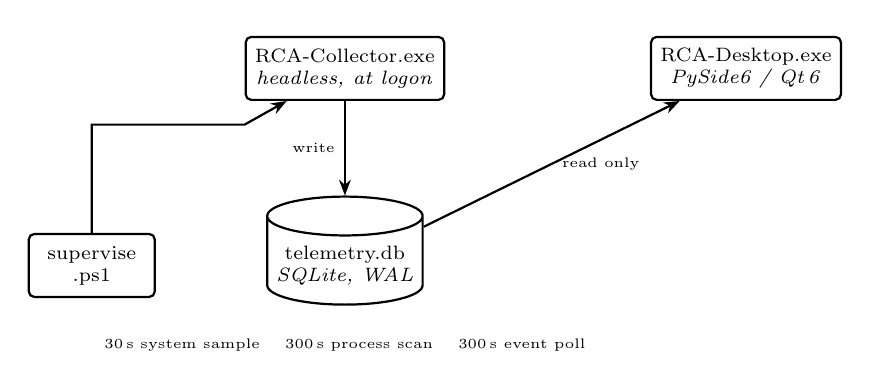
\begin{tikzpicture}[node distance=6mm]
  \node[proc] (coll) {RCA-Collector.exe\\\textit{headless, at logon}};
  \node[store, below=12mm of coll] (db) {telemetry.db\\\textit{SQLite, WAL}};
  \node[proc, right=26mm of coll] (gui) {RCA-Desktop.exe\\\textit{PySide6 / Qt\,6}};
  \node[proc, left=14mm of db, minimum width=16mm] (sup) {supervise\\.ps1};

  \draw[flow] (coll) -- node[left, font=\tiny] {write} (db);
  \draw[flow] (db) -- node[right, font=\tiny] {read only} (gui);
  \draw[flow] (sup) |- ([yshift=-3mm]coll.south west) -- (coll);
  \node[font=\tiny, right=1mm of coll.east, yshift=4mm] {};

  \node[font=\tiny, align=left, below=3mm of db] {%
    30\,s system sample \quad 300\,s process scan \quad 300\,s event poll};
\end{tikzpicture}
\caption{Process architecture. The collector writes; the desktop application
only reads. A PowerShell supervisor restarts the collector if it exits
unexpectedly, because creating a Task Scheduler logon task requires elevation
that a diagnostic tool should not demand.}
\label{fig:arch}
\end{figure}

The collector samples 29 features every 30 seconds, the top processes by CPU
and resident memory every 300 seconds (tightening to 30 seconds under load),
and an allow-listed subset of Windows Event Log records. Retention is
tiered by sensitivity: numeric readings for 365 days, per-process detail for
30 days, and the foreground application name---the most personal field
collected---for 30 days.

%==============================================================================
\section{Method}
\label{sec:method}
%==============================================================================

\subsection{Scaling and windowing}

A min--max scaler is fitted on the clean baseline only,
$x'_j = (x_j - \min_j)/(\max_j - \min_j)$, and incident windows are transformed
with the baseline's parameters and clipped to $[0,1]$. Fitting on the incident
would normalise away the deviation being sought.

Training windows are built \emph{within contiguous segments only}, never
spanning a collection gap. A segment is a maximal run of samples whose spacing
is within tolerance of the sampling cadence.

\subsection{Anomaly detection}

An LSTM autoencoder compresses a window of $T$ samples over $n=29$ features to
a 32-dimensional latent vector and reconstructs it. Only the encoder's final
hidden state reaches the bottleneck, so the entire window is represented by 32
numbers before reconstruction; that compression is the detection mechanism.
Training minimises
\begin{equation}
\mathcal{L} = \frac{1}{B\,T\,n}\sum_{b,t,j}\bigl(x_{btj}-\hat{x}_{btj}\bigr)^2 .
\end{equation}

Error is reduced over time but \emph{not} over features, which is what makes
the output attributable to a metric rather than to a window:
\begin{equation}
s_j = \frac{1}{T}\sum_{t=1}^{T}\bigl(x_{tj}-\hat{x}_{tj}\bigr)^2 .
\end{equation}

Per-metric thresholds are the 99th percentile of validation error,
$\tau_j = P_{99}\{s_j(w)\}$, and a metric is anomalous when $s_j > \tau_j$.
Per-metric thresholds are necessary because reconstructability varies widely:
a near-constant channel reconstructs almost perfectly, while a bursty one does
not, and a single global threshold would flag the latter permanently.

\subsection{Constrained causal inference}

For each ordered pair of anomalous metrics, both series are differenced until
an Augmented Dickey--Fuller test~\cite{dickey1979distribution} rejects a unit
root (at most twice), then
tested for Granger causality at lags $1\ldots L$. The lag minimising the
$p$-value is selected. A pair is skipped unless
\begin{equation}
N \;\ge\; 3L + 2 ,
\label{eq:floor}
\end{equation}
which at the default $L=5$ requires 17 aligned samples. Equation~\eqref{eq:floor}
explains the majority of this system's negative results.

Surviving $p$-values are corrected with Benjamini--Hochberg: sorting ascending,
the largest rank $k$ satisfying $p_{(k)} \le \alpha k / m$ is found and ranks
$1\ldots k$ accepted, with $\alpha = 0.05$. A $p$-value alone is insufficient,
since negligible improvements become significant given a long history, so an
effect-size proxy is also required:
\begin{equation}
\mathrm{effect} = \frac{F}{F+N} \;\ge\; 0.10 .
\end{equation}
This quantity is monotone in $F$, bounded in $(0,1)$, and shrinks as $N$ grows
--- which is the correction desired, since large $N$ is what made the $p$-value
small.

Accepted pairs form a directed graph; cycles are removed preferring edges that
contradict temporal precedence, and remaining edges are filtered against a
subsystem topology prior (Section~\ref{sec:topology}). Candidates are then
ranked by a weighted composite plus PageRank~\cite{page1999pagerank} on the
reversed graph:
\begin{equation}
\mathrm{score}(v) = \min\!\Bigl(1,\; 0.70\!\sum_k w_k s_k(v) \;+\; 0.30\,\mathrm{PR}(v)\Bigr),
\end{equation}
with weights $0.40$ causal outflow, $0.30$ temporal priority, $0.20$ low
inflow, $0.05$ severity and $0.05$ event correlation.

\textbf{A structural caveat.} With zero surviving edges, every node has
outflow $0$ and inflow $1$, so $60\%$ of the weight becomes constant and the
ranking collapses onto severity and timing while still emitting a score. The
system therefore reports the distinction explicitly rather than presenting the
ranking as causal.

\begin{figure}[t]
\centering
\begin{tikzpicture}[node distance=4.5mm]
  \node[term] (start) {incident window};
  \node[step, below=of start] (scale) {scale, clip to $[0,1]$};
  \node[step, below=of scale] (score) {autoencoder: $s_j$ vs $\tau_j$};
  \node[gate, below=of score, minimum width=20mm] (any) {any\\flagged?};
  \node[term, right=10mm of any] (none) {nothing\\anomalous};
  \node[gate, below=8mm of any, minimum width=20mm] (floor) {$N \ge 3L{+}2$?};
  \node[term, right=10mm of floor] (untested) {\textbf{not tested}\\window too short};
  \node[step, below=8mm of floor] (granger) {Granger $\rightarrow$ BH FDR\\$\rightarrow$ effect floor};
  \node[gate, below=of granger, minimum width=20mm] (edges) {edges\\survive?};
  \node[term, right=10mm of edges] (corr) {\textbf{correlation only}\\no causal claim};
  \node[term, below=8mm of edges] (ok) {\textbf{supported}\\ranked chain};

  \draw[flow] (start) -- (scale);
  \draw[flow] (scale) -- (score);
  \draw[flow] (score) -- (any);
  \draw[flow] (any) -- node[above, font=\tiny] {no} (none);
  \draw[flow] (any) -- node[left, font=\tiny] {yes} (floor);
  \draw[flow] (floor) -- node[above, font=\tiny] {no} (untested);
  \draw[flow] (floor) -- node[left, font=\tiny] {yes} (granger);
  \draw[flow] (granger) -- (edges);
  \draw[flow] (edges) -- node[above, font=\tiny] {no} (corr);
  \draw[flow] (edges) -- node[left, font=\tiny] {yes} (ok);
\end{tikzpicture}
\caption{Inference pipeline. Four terminal states are reported distinctly.
Collapsing ``not tested'' into ``nothing survived'' would conflate the absence
of a result with a negative result, which earlier revisions of this system did.}
\label{fig:pipeline}
\end{figure}

%==============================================================================
\section{Evaluation by Fault Injection}
\label{sec:eval}
%==============================================================================

Because a personal machine provides no labelled incidents, we manufacture
ground truth: a harness causes a specific, known disturbance, waits for
samples to land at the real cadence, runs the production pipeline over the
injection window, and scores the result.

\begin{table}[t]
\caption{Controlled fault injections, 30-minute windows unless noted}
\label{tab:injection}
\centering
\footnotesize
\begin{tabular}{@{}llccl@{}}
\toprule
\textbf{Fault} & \textbf{Samples} & \textbf{Flagged} & \textbf{Edges} & \textbf{Outcome} \\
\midrule
CPU, 7\,min      & 14 & 6/29 & --- & not tested (below floor) \\
CPU              & 60 & 6/29 & \textbf{6} & \textbf{explained correctly} \\
Disk             & 60 & 4/29 & 0 & detected, unexplained \\
Memory           & 60 & 2/29 & 0 & wrong process named \\
Memory (refixed) & 60 & 3/29 & 0 & detected, attributed \\
Memory (clean)   & 60 & 0/29 & --- & not measurable on host \\
Idle             & 60 & 1/29 & --- & 3.4\% false positives \\
\bottomrule
\end{tabular}
\end{table}

\subsection{A correct explanation of an unknown cause}

Half the CPU cores were burned for 30 minutes with no information given to the
pipeline. The ranking named \texttt{cpu\_pct} first at $1.000$, and the
surviving edges are oriented \emph{away} from CPU---the signature of a genuine
root cause, since nothing upstream drives it:
\[
\texttt{cpu\_pct\_max\_core} \rightarrow \texttt{disk\_busy\_pct}
\quad (\text{lag } 2,\ 0.756).
\]

\subsection{Starvation, not failure}

The same fault at 7 and at 30 minutes differed only in duration. At 14 samples,
against the floor of 17 from~\eqref{eq:floor}, \emph{no pair was compared at
all}, and the system reported exactly that. At 60 samples, ten pairs survived
correction and six survived the topology filter. The causal layer was not
broken; it was starved. This distinction changes the remedy from redesign to
window width, and is confirmed at scale in Section~\ref{sec:population}.

\subsection{A defect that injection exposed}

The memory injection detected the anomaly and then attributed it to four
unrelated processes. Attribution ranked candidates by mean CPU, while resident
memory was selected but never sorted on---so a process that allocates and
sleeps could never be named. A memory-bound cause was unreportable
\emph{by construction}, in every incident the system had ever analysed. The
CPU and disk faults are both CPU-heavy and had attributed correctly by
accident of their shape, concealing the defect.

\subsection{A measurement this host cannot provide}

A later memory injection on a deliberately cleared machine flagged nothing.
The detector was correct: the host's median memory utilisation across 30{,}199
samples is $95.2\%$, and the injection window sat at $87.4\%$---the 9th
percentile of its own history. The injection is bounded to half of free memory
for safety, which on a habitually-full host cannot exceed the level the machine
already reaches unaided. The fault is undetectable \emph{by construction} here,
and the harness now reports this as inconclusive rather than as a detector
failure.

%==============================================================================
\section{Population-Scale Evaluation}
\label{sec:population}
%==============================================================================

Fault injection establishes correctness on a handful of cases but yields single
observations. To measure \emph{frequency}, the pipeline was replayed over every
incident discoverable in real collected history---no injection, read-only.

\begin{figure}[t]
\centering
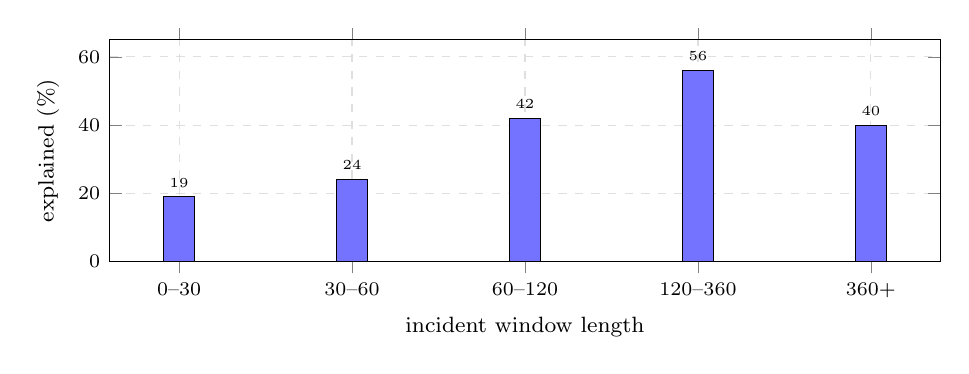
\begin{tikzpicture}
\begin{axis}[
  width=\columnwidth, height=4.4cm,
  ybar, bar width=11pt,
  ymin=0, ymax=65,
  ylabel={\footnotesize explained (\%)},
  xlabel={\footnotesize incident window length},
  symbolic x coords={0--30,30--60,60--120,120--360,360+},
  xtick=data,
  tick label style={font=\scriptsize},
  label style={font=\scriptsize},
  nodes near coords, every node near coord/.append style={font=\tiny},
  grid=major, grid style={dashed,gray!25},
]
\addplot[fill=blue!55] coordinates
  {(0--30,19) (30--60,24) (60--120,42) (120--360,56) (360+,40)};
\end{axis}
\end{tikzpicture}
\caption{Causal yield against window length, over 113 analysable incidents.
The rate roughly doubles once windows exceed one hour, confirming at scale the
starvation effect first seen in a single pair of injections. The final bar
represents five incidents and should not be read as a downward trend.}
\label{fig:yield}
\end{figure}

Of $210$ incidents discovered, $97$ ($46\%$) fall below the sample floor of
\eqref{eq:floor} and cannot be tested at any setting. Of the $113$ that can be,
$30$ produce a supported causal chain. The end-to-end figure a user experiences
is therefore $30/210 = 14.3\%$: roughly one incident in seven receives a causal
explanation.

We report the funnel rather than the survivor-filtered rate. The share of
\emph{analysable} incidents explained is $26.5\%$, which is the more flattering
number and describes fewer situations.

\textbf{The floor is a parameter artefact.} Short incidents are widened before
analysis to exactly the model's window size, 15 samples, while~\eqref{eq:floor}
at $L=5$ requires 17---two constants chosen independently in the same pipeline.
Re-running the survey at $L\in\{3,4,5\}$ over an identical population shows the
cliff disappears at $L\le4$, but recovers little: explanations rise only from
$30$ to $34$ while the tested population nearly doubles, and median surviving
edges falls from $2$ to $1$. The gain is honest reporting---``tested, nothing
found'' instead of ``not tested''---rather than insight.

%==============================================================================
\section{Auditing the Subsystem Prior}
\label{sec:topology}
%==============================================================================

Since no service call graph exists on an endpoint, the system encodes domain
knowledge as an explicit map of permissible subsystem influence. Auditing it
across all analysable incidents shows it is the largest single filter in the
pipeline after the statistical gates: of $115$ accepted pairs, $65$ survive,
$30$ ($26\%$) are rejected by the map and $20$ ($17\%$) by cycle-breaking.

\begin{figure}[t]
\centering
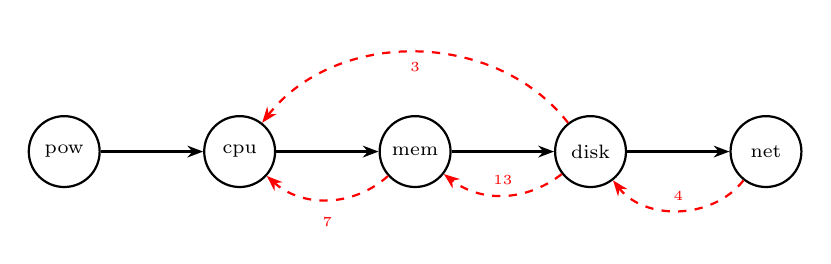
\begin{tikzpicture}[node distance=13mm]
  \node[subsys] (pow) {pow};
  \node[subsys, right=of pow] (cpu) {cpu};
  \node[subsys, right=of cpu] (mem) {mem};
  \node[subsys, right=of mem] (dsk) {disk};
  \node[subsys, right=of dsk] (net) {net};

  \draw[flow] (pow) -- (cpu);
  \draw[flow] (cpu) -- (mem);
  \draw[flow] (mem) -- (dsk);
  \draw[flow] (dsk) -- (net);

  \draw[flow, red, dashed] (dsk) to[bend left=38] node[above, font=\tiny] {13} (mem);
  \draw[flow, red, dashed] (mem) to[bend left=42] node[below=1mm, font=\tiny] {7} (cpu);
  \draw[flow, red, dashed] (net) to[bend left=52] node[above, font=\tiny] {4} (dsk);
  \draw[flow, red, dashed] (dsk) to[bend right=52] node[below, font=\tiny] {3} (cpu);
\end{tikzpicture}
\caption{The subsystem prior is a strict total order (solid), so
\texttt{network} is a sink and nothing can be reported as caused by network
activity. Dashed edges are directions the statistics accepted and the map
rejected, labelled with occurrence counts. Three of them describe real
mechanisms: a download writing to disk, the file cache consuming memory, and
interrupt handling costing CPU.}
\label{fig:topology}
\end{figure}

Every rejected transition has \emph{zero} survivors, because the map forbids
whole classes rather than individual edges (Fig.~\ref{fig:topology}). Judged
individually, \texttt{network}\,$\rightarrow$\,\texttt{disk} is almost certainly
real---a download arrives over the network and is written to disk---and the
strongest single relationship measured anywhere in this work, at $0.982$, is
exactly this pair. \texttt{disk}\,$\rightarrow$\,\texttt{memory} reflects the
Windows standby file cache, and \texttt{disk}\,$\rightarrow$\,\texttt{cpu}
reflects interrupt and DPC handling. Conversely,
\texttt{memory}\,$\rightarrow$\,\texttt{process} cleared the effect floor by
$0.009$ and is plausibly spurious.

The prior is therefore not so much wrong as \emph{one-directional}: it models
resource pressure flowing downhill and has no vocabulary for the feedback that
makes I/O expensive. Adding the reverse edges would make the graph cyclic,
where cycle-breaking already removes $17\%$ of pairs---so the two mechanisms
would begin to compete. We record this as an open design question rather than
patching it.

%==============================================================================
\section{Discussion and Threats to Validity}
%==============================================================================

\textbf{All measurements come from one machine.} Nothing here establishes
generality, and one measurement---memory-fault detection---is provably
unobtainable on this host, which makes second hardware a prerequisite rather
than an enhancement.

\textbf{Correctness is not established at population scale.} The survey's 210
incidents have no known cause, so a $14.3\%$ explanation rate reports how often
the layer speaks, never whether it is right. The rate is a ceiling on
usefulness, not a measure of accuracy.

\textbf{No fault has been tested whose cause is not also the loudest metric.}
Both explaining runs put the injected fault atop a severity ranking, so a
correct causal answer and a correct severity answer remain indistinguishable.

\textbf{Granger causality is not causation.} It is correlation under a temporal
constraint. The FDR correction, effect floor and subsystem prior exist to
suppress the resulting over-reporting, and Section~\ref{sec:topology} shows the
prior itself is imperfect.

\textbf{A methodological observation.} Nine defects were found in code carrying
a passing test suite of 130 tests. In nearly every case the test asked a
question \emph{adjacent} to the one that mattered---a database value instead of
the bytes on disk, one file instead of the full storage footprint, a function
instead of the code path calling it. Two fixes were worse than the defects they
repaired. These were caught by adversarial review rather than additional
testing, which we believe generalises beyond this system.

%==============================================================================
\section{Conclusion}
%==============================================================================

We presented an on-device root cause analysis system for Windows endpoints
operating without ground truth, network access or fleet context. Under
controlled injection it detects and attributes CPU, disk and memory faults, and
has produced a correct causal explanation of a fault it was never told about.
Across real history it explains roughly one incident in seven, declines to
explain the rest, and distinguishes ``not tested'' from ``tested and nothing
survived''.

We argue this last property matters more than the explanation rate. A tool
reporting ``no causal chain was supported'' when the data cannot support one is
more useful than a confident ranking that changes with the analysis window---and
in this system, the engineering required to make it say so honestly exceeded
the engineering required to compute an answer at all.

Future work: repeating the evaluation on second hardware, testing a fault whose
cause is not the loudest metric, and resolving whether the subsystem prior
should admit the feedback directions it currently forbids.

%==============================================================================
\begin{thebibliography}{00}

\bibitem{malhotra2016lstm}
P.~Malhotra, A.~Ramakrishnan, G.~Anand, L.~Vig, P.~Agarwal, and G.~Shroff,
``LSTM-based encoder-decoder for multi-sensor anomaly detection,'' in
\emph{Proc. ICML Anomaly Detection Workshop}, 2016.

\bibitem{hundman2018detecting}
K.~Hundman, V.~Constantinou, C.~Laporte, I.~Colwell, and T.~Soderstrom,
``Detecting spacecraft anomalies using LSTMs and nonparametric dynamic
thresholding,'' in \emph{Proc. ACM SIGKDD}, 2018, pp. 387--395.

\bibitem{granger1969investigating}
C.~W.~J. Granger, ``Investigating causal relations by econometric models and
cross-spectral methods,'' \emph{Econometrica}, vol.~37, no.~3, pp. 424--438,
1969.

\bibitem{benjamini1995controlling}
Y.~Benjamini and Y.~Hochberg, ``Controlling the false discovery rate: a
practical and powerful approach to multiple testing,'' \emph{J. Roy. Statist.
Soc. B}, vol.~57, no.~1, pp. 289--300, 1995.

\bibitem{kim2013root}
M.~Kim, R.~Sumbaly, and S.~Shah, ``Root cause detection in a service-oriented
architecture,'' in \emph{Proc. ACM SIGMETRICS}, 2013, pp. 93--104.

\bibitem{chen2014causeinfer}
P.~Chen, Y.~Qi, P.~Zheng, and D.~Hou, ``CauseInfer: automatic and distributed
performance diagnosis with hierarchical causality graph in large distributed
systems,'' in \emph{Proc. IEEE INFOCOM}, 2014, pp. 1887--1895.

\bibitem{page1999pagerank}
L.~Page, S.~Brin, R.~Motwani, and T.~Winograd, ``The PageRank citation ranking:
bringing order to the web,'' Stanford InfoLab, Tech. Rep. 1999-66, 1999.

\bibitem{dickey1979distribution}
D.~A. Dickey and W.~A. Fuller, ``Distribution of the estimators for
autoregressive time series with a unit root,'' \emph{J. Amer. Statist. Assoc.},
vol.~74, no.~366, pp. 427--431, 1979.

\end{thebibliography}

\end{document}
